\documentclass[final, xcolor={table,dvipsnames},t]{beamer}

% ====================
% Packages
% ====================
\usepackage[T1]{fontenc}
\usepackage{lmodern}
\usepackage[size=custom, width=122,height=91, scale=1.2]{beamerposter} % Current dimensions A0, put in your poster dimensions
\usetheme[Blue]{UVic} % Options are DarkBlue, Blue, or White, all themed with UVic Edge styling
\usepackage{graphicx}
\usepackage{caption}
\usepackage{booktabs}
\usepackage{tikz}
\usepackage{pgfplots}
\pgfplotsset{compat=1.14}
\newcommand{\blu}{\color{blue}}
\usepackage{anyfontsize}
\usepackage{tikz}
\usetikzlibrary{automata, positioning, arrows}
\usepackage{subfigure}

\usepackage{blindtext}


%%%%%%%%%%%%%%%%%%%%%%%%%%%%%%%%%%%%%%%%%%%%%%%%%%%%%%%%%%%%%%%%%%%%%%%%%%%%%%
% Column environment setup
%%%%%%%%%%%%%%%%%%%%%%%%%%%%%%%%%%%%%%%%%%%%%%%%%%%%%%%%%%%%%%%%%%%%%%%%%%%%%%
% If you have N columns, choose \sepwidth and \colwidth such that
% (N+1)*\sepwidth + N*\colwidth = \paperwidth
\newlength{\sepwidth}
\newlength{\colwidth}
\setlength{\sepwidth}{0.025\paperwidth}
\setlength{\colwidth}{0.3\paperwidth}

\newcommand{\separatorcolumn}{\begin{column}{\sepwidth}\end{column}}

% You can also use these column commands to create columns inside columns and for creating new column formatting. 
% You can also have non even columns by creating more column environments or specifying the width when beginning a column environment. 
%%%%%%%%%%%%%%%%%%%%%%%%%%%%%%%%%%%%%%%%%%%%%%%%%%%%%%%%%%%%%%%%%%%%%%%%%%%%%%
% Title
%%%%%%%%%%%%%%%%%%%%%%%%%%%%%%%%%%%%%%%%%%%%%%%%%%%%%%%%%%%%%%%%%%%%%%%%%%%%%%

\title{\VeryHuge{Smart Parking Guidance System}}
\author{\textbf{Ruilin Wang}, Yun Ma and Oche Eko}
\institute[shortinst]{University of Victoria, Department of Electricl and Computer Engineering}

%%%%%%%%%%%%%%%%%%%%%%%%%%%%%%%%%%%%%%%%%%%%%%%%%%%%%%%%%%%%%%%%%%%%%%%%%%%%%%
% Poster footer
%%%%%%%%%%%%%%%%%%%%%%%%%%%%%%%%%%%%%%%%%%%%%%%%%%%%%%%%%%%%%%%%%%%%%%%%%%%%%%

\footercontent{
  \href{https://github.com/wanrylin/Smart-Parking-Guidance-System}{Github: https://github.com/wanrylin/Smart-Parking-Guidance-System} \hfill
ECE 514 Design and Analysis of Communication Networks Course Project \hfill
  \href{ruilinwang@uvic.ca}{ruilinwang@uvic.ca}} 

\begin{document}
%%%%%%%%%%%%%%%%%%%%%%%%%%%%%%%%%%%%%%%%%%%%%%%%%%%%%%%%%%%%%%%%%%%%%%%%%%%%%%
% Logo placements (optional)
%%%%%%%%%%%%%%%%%%%%%%%%%%%%%%%%%%%%%%%%%%%%%%%%%%%%%%%%%%%%%%%%%%%%%%%%%%%%%%

% \addtobeamertemplate{headline}{}
% {
%     \begin{tikzpicture}[remember picture,overlay,line width=\arrayrulewidth]
%     %   Logo in top right below header
%       \node [anchor=north east, inner sep=3cm] at ([xshift=1.0cm,yshift=-10.0cm]current page.north east)
%       {\includegraphics[height=6.0cm]{logos/mylogo.eps}}; 
%         % Logo in top left below header
%       \node [anchor=north west, inner sep=3cm] at ([xshift=-1.0cm,yshift=-10.0cm]current page.north west)
%       {\includegraphics[height=7.0cm]{logos/mylogo.eps}}; 
%     \end{tikzpicture}
% }

% ====================
% Body
% ====================

\begin{frame}[t]
\begin{columns}[t]
\separatorcolumn

\begin{column}{\colwidth}

  \begin{block}{Motivation}
  Currently, numerous universities are encountering the following challenges in managing parking within their campuses: 

    \begin{itemize}
      \item \textbf{Growing Demand:} \\In an auto-dependent society like Canada, the demand for parking spaces intensifies as college populations increase.
      \item \textbf{Environmental and Financial Considerations:}\\ Valuable resources such as gasoline and time are wasted in searching for available parking spaces.
      \item \textbf{Land Use Conflicts:}\\ The growth in college populations leads to conflicts between the need for parking spaces and other land uses.
    \end{itemize}
  \end{block}

  \begin{block}{Challenges}
  
    \begin{itemize}
      \item \textbf{Parking lot occupancy prediction:}\\ Based on the current parking situation, predicting the future occupancy of parking facilities over a specified period.
      \item \textbf{Traffic Control:}\\ Balance the occupancy of each parking lot and prevent congestion.
      \item \textbf{Parking Route Optimization:}\\ Minimize time spent in the parking lot and on the way to the destination.
    \end{itemize}

  \end{block}

  \begin{alertblock}{Theoretical Model for Parking Lot}
    The future occupancy of the parking spots depends on the present occupancy but not on past occupancies, which can be expressed as 
    \begin{equation*}
        \Pr[X(t + s) = u|X(s) = v, X(s_1) = w_1, \ldots, X(s_n) = w_n] = \Pr[X(t + s) = u|X(s) = v]
    \end{equation*}

    Therefore, we can model the parking lot occupancy into a \textbf{M/M/s/s} queue model, where $s$ is the number of parking place in a parking lot\cite{predicting}. The vehicle influx to the parking facility follows a Poisson distribution characterized by an arrival rate $\lambda$. Assuming each vehicle takes one parking slot, the duration for occupied space adheres to an exponential distribution with a parking rate $\mu$, the inverse of paring time. 

    The state transitions of this parking lot model are given by

    \begin{center}
    \begin{tikzpicture}[node distance=2cm and 2cm, auto,>=latex', thick]
    % Nodes
    \node[state] (s0) {0};
    \node[state, right=of s0] (s1) {1};
    \node[state, right=of s1] (s2) {2};
    \node[right=of s2] (sdots) {$\ldots$};
    \node[state, right=of sdots] (sn) {s};

    % Paths
    \path[->] (s0) edge[bend left] node {$\lambda$} (s1);
    \path[->] (s1) edge[bend left] node {$\lambda$} (s2);
    \path[->] (s2) edge[bend left] node[above] {$\lambda$} (sdots);
    \path[->] (sdots) edge[bend left] node[above] {$\lambda$} (sn);
    
    \path[->] (s1) edge[bend left] node[below] {$\mu$} (s0);
    \path[->] (s2) edge[bend left] node[below] {$2\mu$} (s1);
    \path[->] (sdots) edge[bend left] node[below] {$3\mu$} (s2);
    \path[->] (sn) edge[bend left] node[below] {$s\mu$} (sdots);
\end{tikzpicture}      
    \end{center}

    If we express this in the form of a transition matrix $Q$, we obtain
    \begin{equation*}
        Q = \begin{pmatrix}
-\lambda & \lambda & 0 & \dots & 0 \\
\mu & -(\lambda + \mu) & \lambda & \dots & 0 \\
0 & 2\mu & -(\lambda + 2\mu) & \dots & 0 \\
\vdots & \vdots & \vdots & \ddots & \vdots \\
0 & \vdots & (s -1)\mu & -(\lambda + (s - 1)\mu) & \lambda\\
0 & 0 & \dots & s\mu & -s\mu \\
\end{pmatrix}
    \end{equation*}

    For M/M/s/s queue model, the parking lot can be modeled as $M(t,s,o,\lambda,\mu)$, where $t$ is current time and $o$ is the occupied parking space\cite{finding}. The probability distribution at state o and time $t$ is defined as $\pi(t)$. Then the probability distribution of the occupancy number after $k$ time step is given by
    \begin{equation*}
        \pi (t + k) = \pi (t) e^{kQ}
    \end{equation*}
    

  \end{alertblock}

\end{column}

\separatorcolumn

\begin{column}{\colwidth}

  \begin{block}{Recommendation System}
    To predict the total time consumed from when vehicles arrive on campus to when users reach their final building, two aspects are considered: parking time and walking time. 

    \begin{enumerate}
      \item \textbf{Parking Time:}\\ This counts the time consumed from user drive in the parking lot to it parks the car. The value of this metric highly related to the size and occupied rate of parking lot. It can be modeled as:
      \begin{equation*}
          T = e^{ln(1 + \frac{s}{120})\alpha}
      \end{equation*}
      where $s$ is the total parking space in the parking lot and $\alpha = \frac{o}{s}$ is occupied rate. 
      \item \textbf{Walk Time:}\\ This counts the time consumed on the way user walking to its terminated building in the campus, which can be obtained from online source like Google Map.
    \end{enumerate}

    The working flow of this recommendation system is shown here.
    \begin{figure}[H]
	\centering
	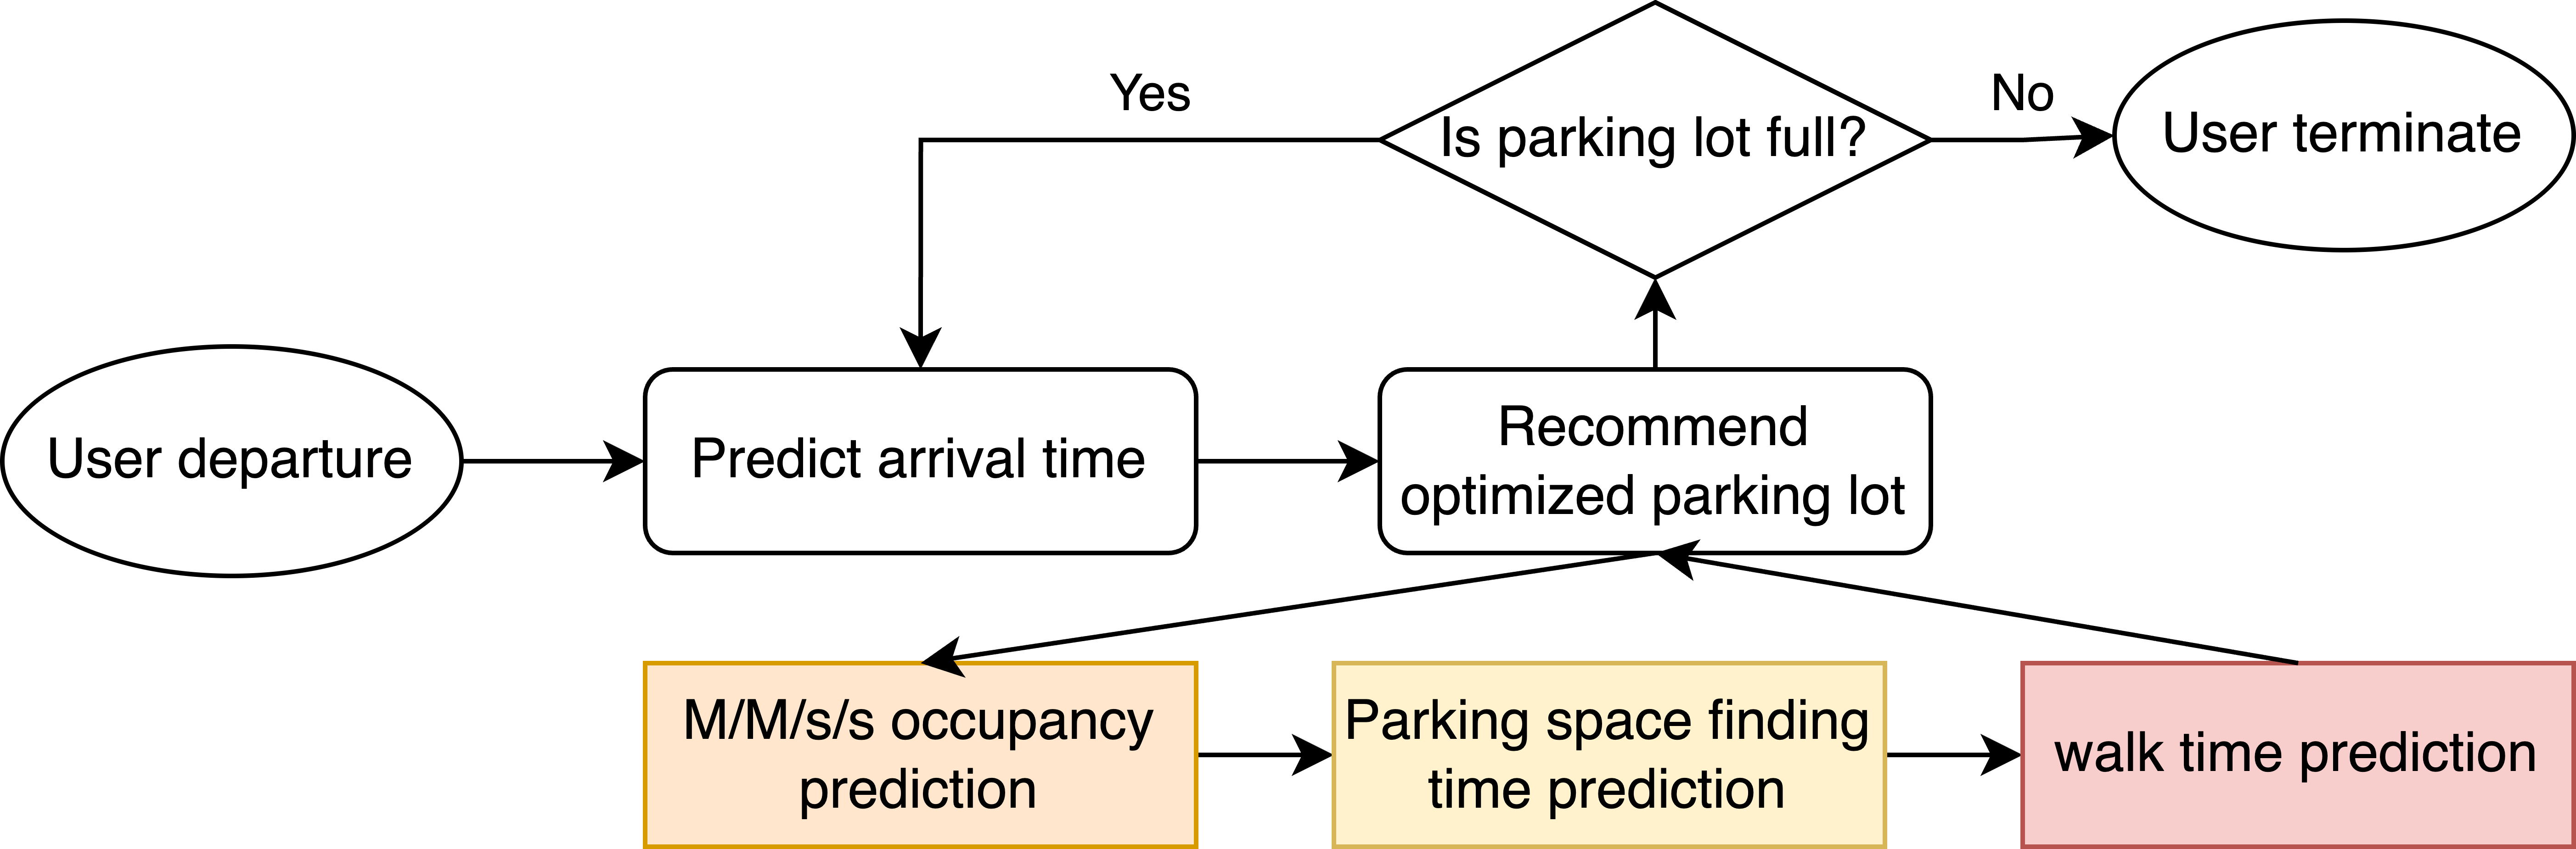
\includegraphics[scale=2]{ECE514.png}
	% \caption{the decision line of $\eta=100$ }
	\label{work flow}
    \end{figure}

  \end{block}

  \begin{block}{Data Model}

   The University of Victoria (UVic), located in Victoria, British Columbia, is the province's oldest tertiary institution with 22020 students and 5000 staff members.From survey, 37.6\% individual using cars for transportation in 2018\cite{UVic2018TransportationSurvey}.


    \begin{itemize}
      \item \textbf{course enrollments} According to the trip chaining patterns of Eomet al. (2009)\cite{managing}, there is a correlation between course enrollments and campus parking. To simulate the demand of parking lot, we collected three sets of data: course enrollment data, facility information and campus parking lot space.


        \begin{itemize}
          \item Course enrollment data for 2023 to 2024 were obtained from Online Tools of UVic. This data provide location, time, course length and class size information.

          






        


          \item Classes are usually scheduled at certain times: between 9 and 10 in the morning, 11 and 12, or 1 and 3 in the afternoon. This happens for a few reasons. Teachers might pick these times because they work best with their own schedules or other jobs. These times are chosen instead of early morning, late afternoon, or evening. Also, having classes at these times might help more students to attend.

          
        \end{itemize}
      
    \end{itemize}

    \begin{itemize}
      \item \textbf{parking demand}  Students often come to campus before their class starts or stay after for different reasons, like meeting other students, visiting professors during office hours, or using the library. This idea is backed by research from Eom et al. (2009)\cite{managing}. 


        \begin{itemize}
          \item Formulation for the relationship between course number and k-hour windows of a certain period.
        $$ EE_{(t,k)} = \sum_{T=(t-k)}^{t+k} E_T $$
        $ E_t = $ the total course enrollment on campus at time t.
          \item According to the University of Victoria's 2018 Transportation Survey, there is a strongest correlation between time spent on campus and course enrollment size occurs with a 2-hour window (k = 2). This means that students tend to come to campus about two hours before their class starts or stay for two hours after it ends. They do this for different reasons related to their courses or for social activities.
        $$Demand_t = a_1\cdot S + a_2 EE_{t,2} + \lambda$$
        $Demand_t =$ number of demand parking space at time t in campus
        $a_1 =$ the proportion of car users within UVic
        $S =$ number of parking space in campus
        $EE_{t,2} =$ number of courses within 2-hour time window at time t
        $\lambda =$ Error term
          \item Donec rhoncus vestibulum erat, quis aliquam leo
            gravida egestas.
        \end{itemize}
      
    \end{itemize}





  \end{block}

\end{column}

\separatorcolumn

\begin{column}{\colwidth}

  \begin{exampleblock}{Demo: UVic Campus Parking Guidance System}

\heading{Implementation Scenario}
\begin{figure}[h]
    \centering
    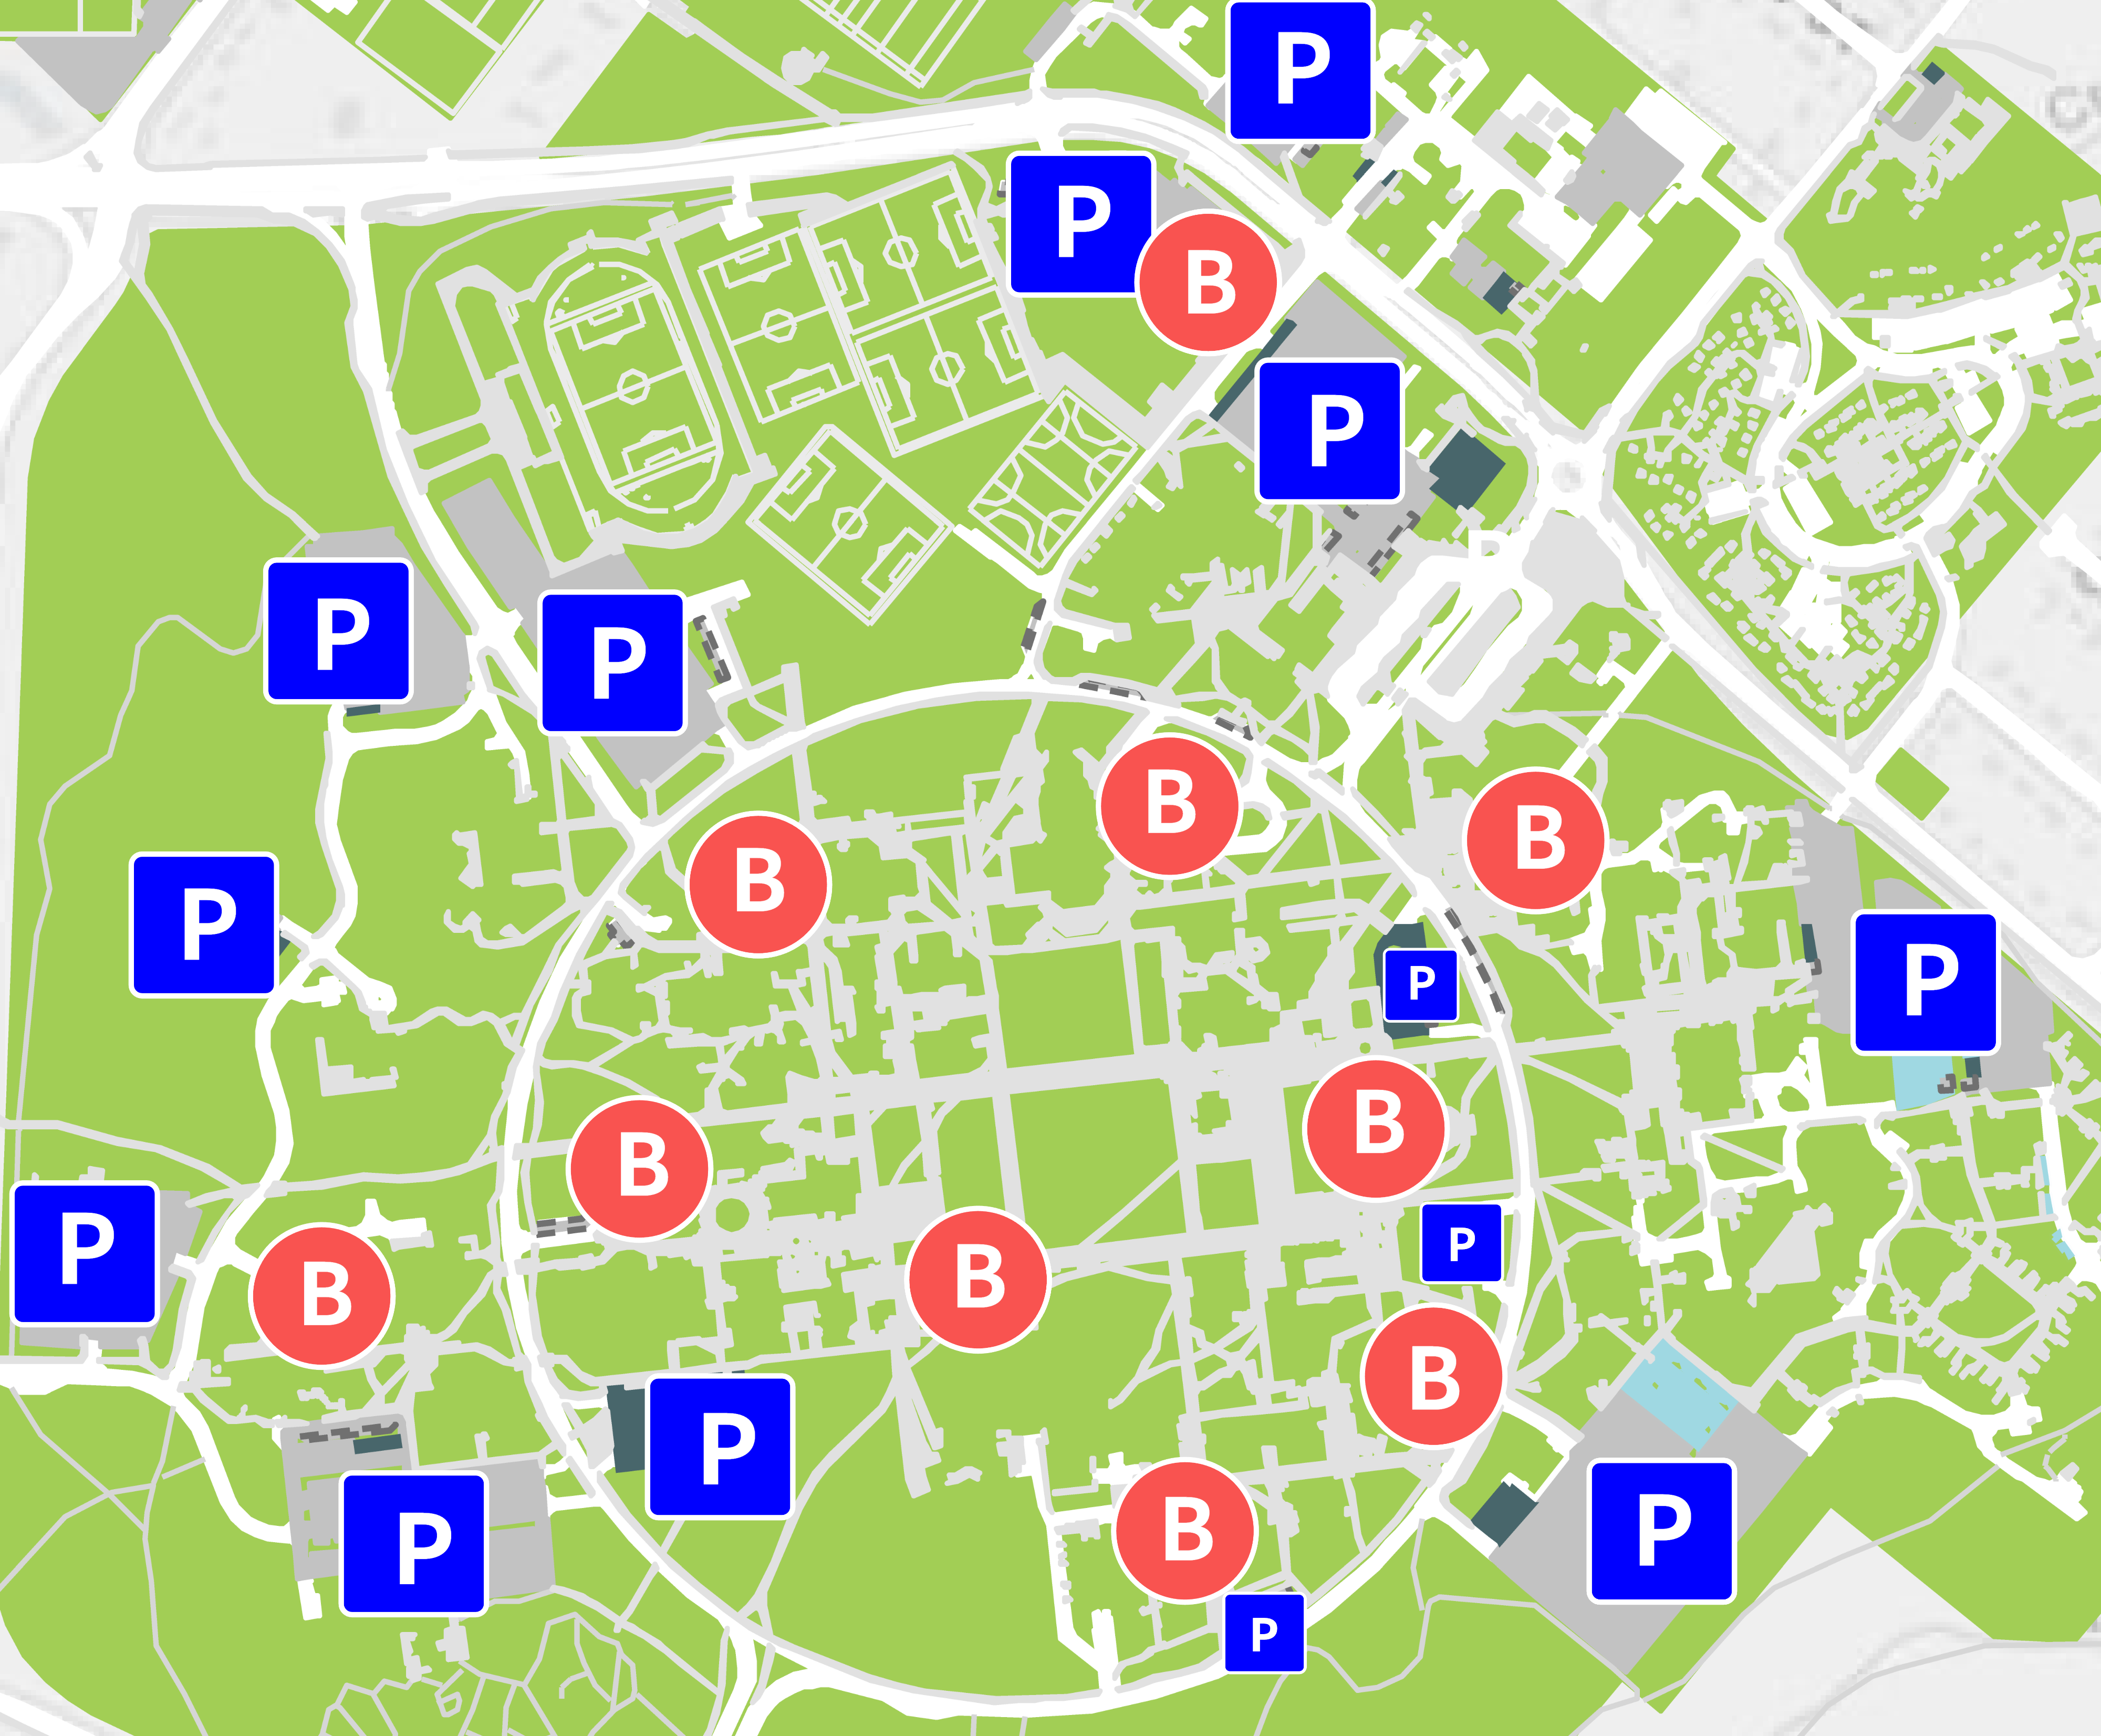
\includegraphics[width=0.45\textwidth]{CampusMap.png} 
    \hfill 
    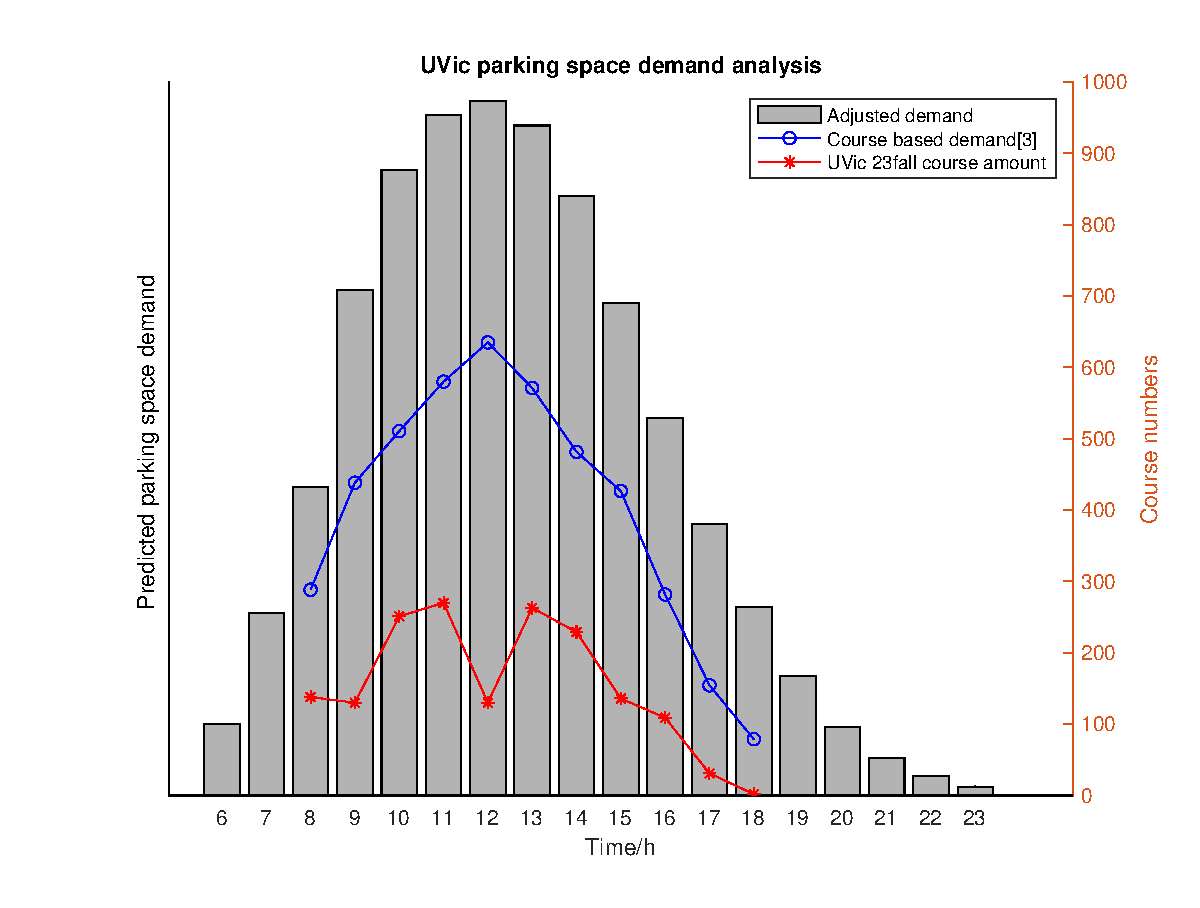
\includegraphics[width=0.45\textwidth]{dataset.eps}
    \label{performance} 
\end{figure}
    We simulate proposed system in the condition of UVic campus. In total, 14 parking lots and 10 buildings are selected as the representation for simulation. \\
    Parking lot includes: Lot 1-10, Lot A,B,C,E. Building includes: McPherson Library, CARSA, SUB, BWC, ELW, CUN, Visual Arts Department Builiding, Human & Social Department Building, David Turpin Building and Jamie Cassels Centre.

    \heading{Dataset}
    According to data model, we generated 10000 data samples. Each data sample is a $1\times4$ vector, which contains departure time, arrival time, leave time, destination building. For each simulation, we randomly pick some of them to run the system.
  \end{exampleblock}

  \begin{block}{Performance Evaluation}

\begin{figure}[h]
    \centering
    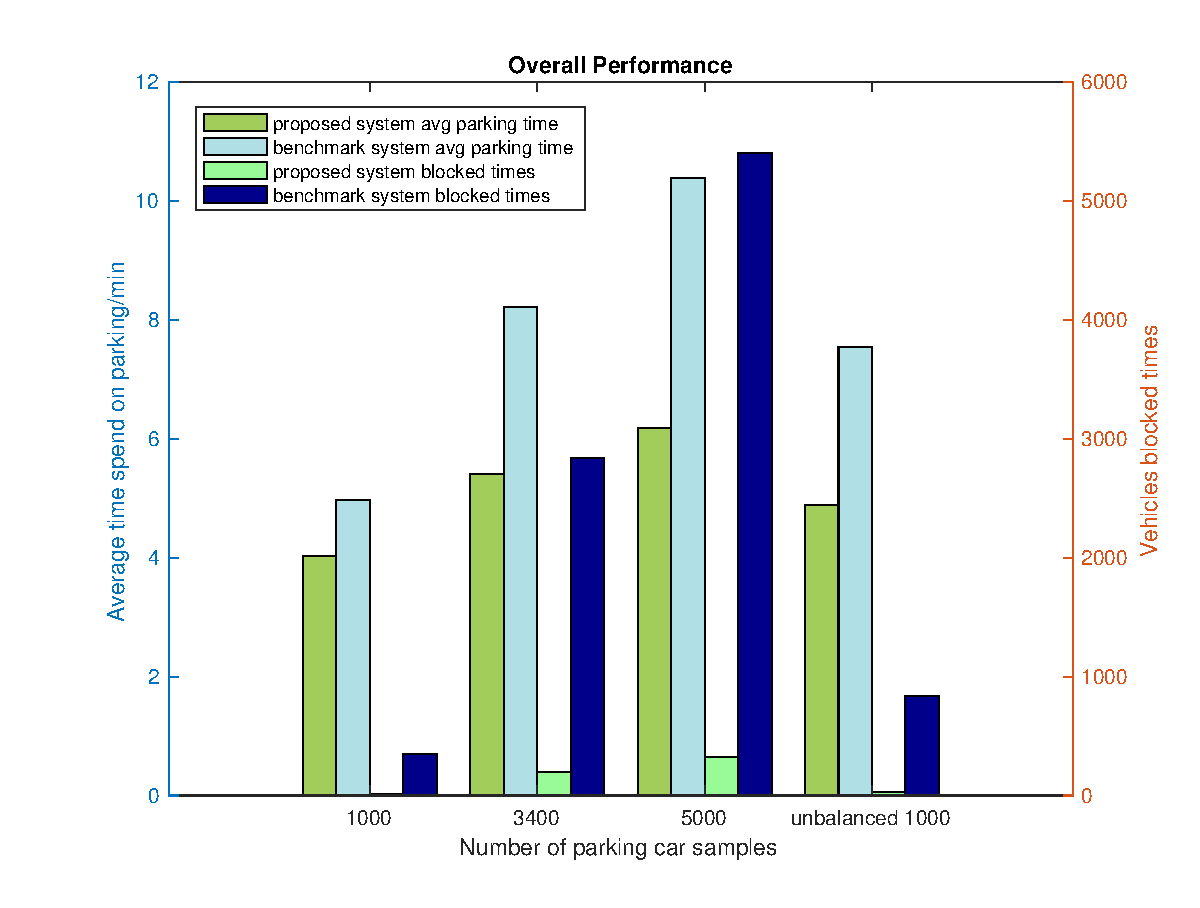
\includegraphics[width=0.45\textwidth]{overall.eps} 
    \hfill 
    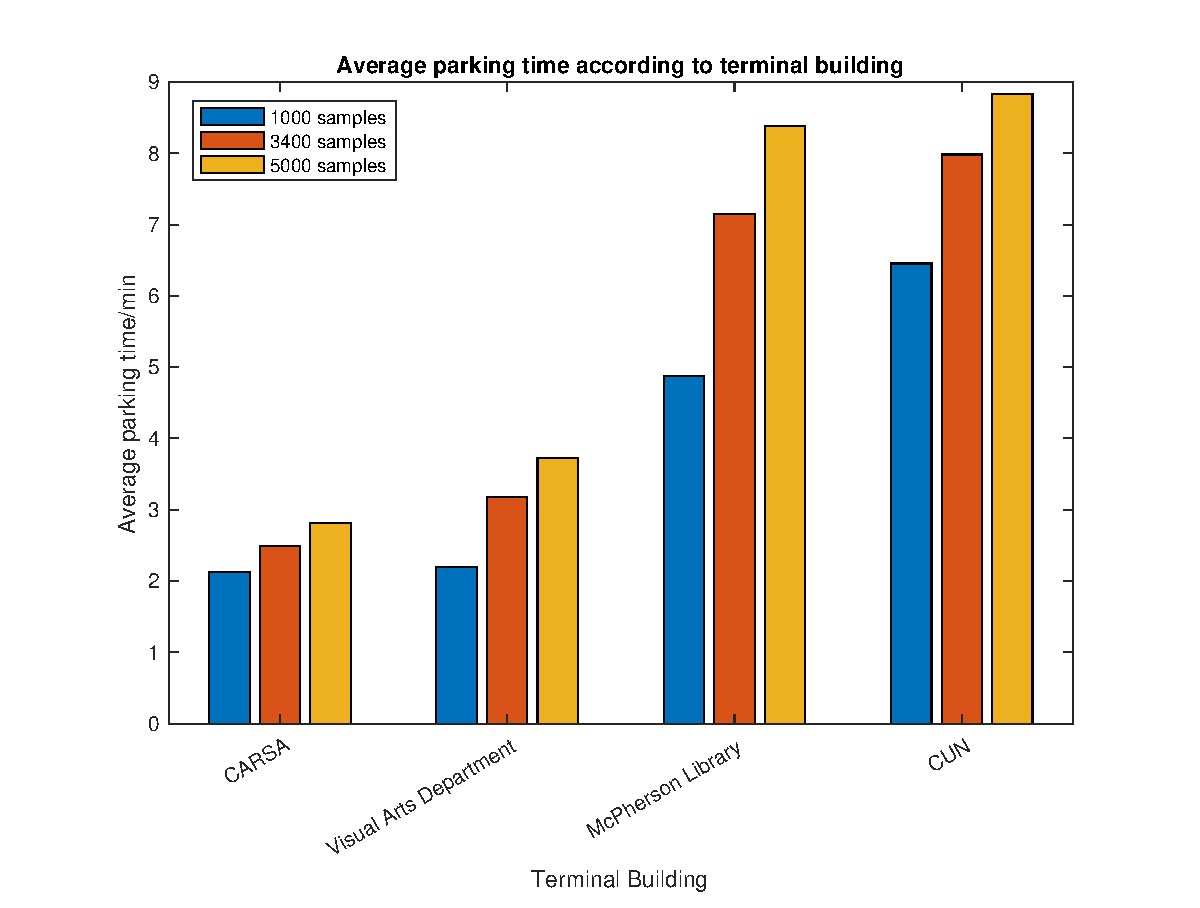
\includegraphics[width=0.45\textwidth]{parkinglot.eps} 
    \label{performance} 
\end{figure}
Benchmark assumes user always choose the parking lot closest to its destination.


  \end{block}

  \begin{block}{Conclusion}
    \begin{itemize}
      \item \textbf{Contribution:} Compared to benchmark, the proposed system brings 20\% to 40\% time and fuel waste decrease. It shows robustness when managing heavy traffic or unbalanced demand.
      \item \textbf{Suggestion:}  From the simulation result, people whose terminal is CUN and Library area spend longest time on parking. For future plan, new parking lot should take more consideration about CUN and Library convenience. 
    \end{itemize}
      
  \end{block}

  \begin{block}{References}

    \nocite{*}
    \scriptsize{\bibliographystyle{plain}\bibliography{poster}}

  \end{block}

\end{column}

\separatorcolumn
\end{columns}
\end{frame}

\end{document}